% ============================================
% Chapitre 6 : Monitoring et Tableaux de Bord
% ============================================
\chapter{Monitoring et Tableaux de Bord}
\label{chap:monitoring}

\section{Vue d'Ensemble du Monitoring}

Une fois les agents configurés et connectés, Zabbix collecte automatiquement les métriques des hôtes supervisés. Cette section présente les fonctionnalités de monitoring et de visualisation.

\section{Dashboard Principal}

Le tableau de bord principal de Zabbix affiche une vue synthétique de l'état de l'infrastructure :

\begin{figure}[H]
\centering
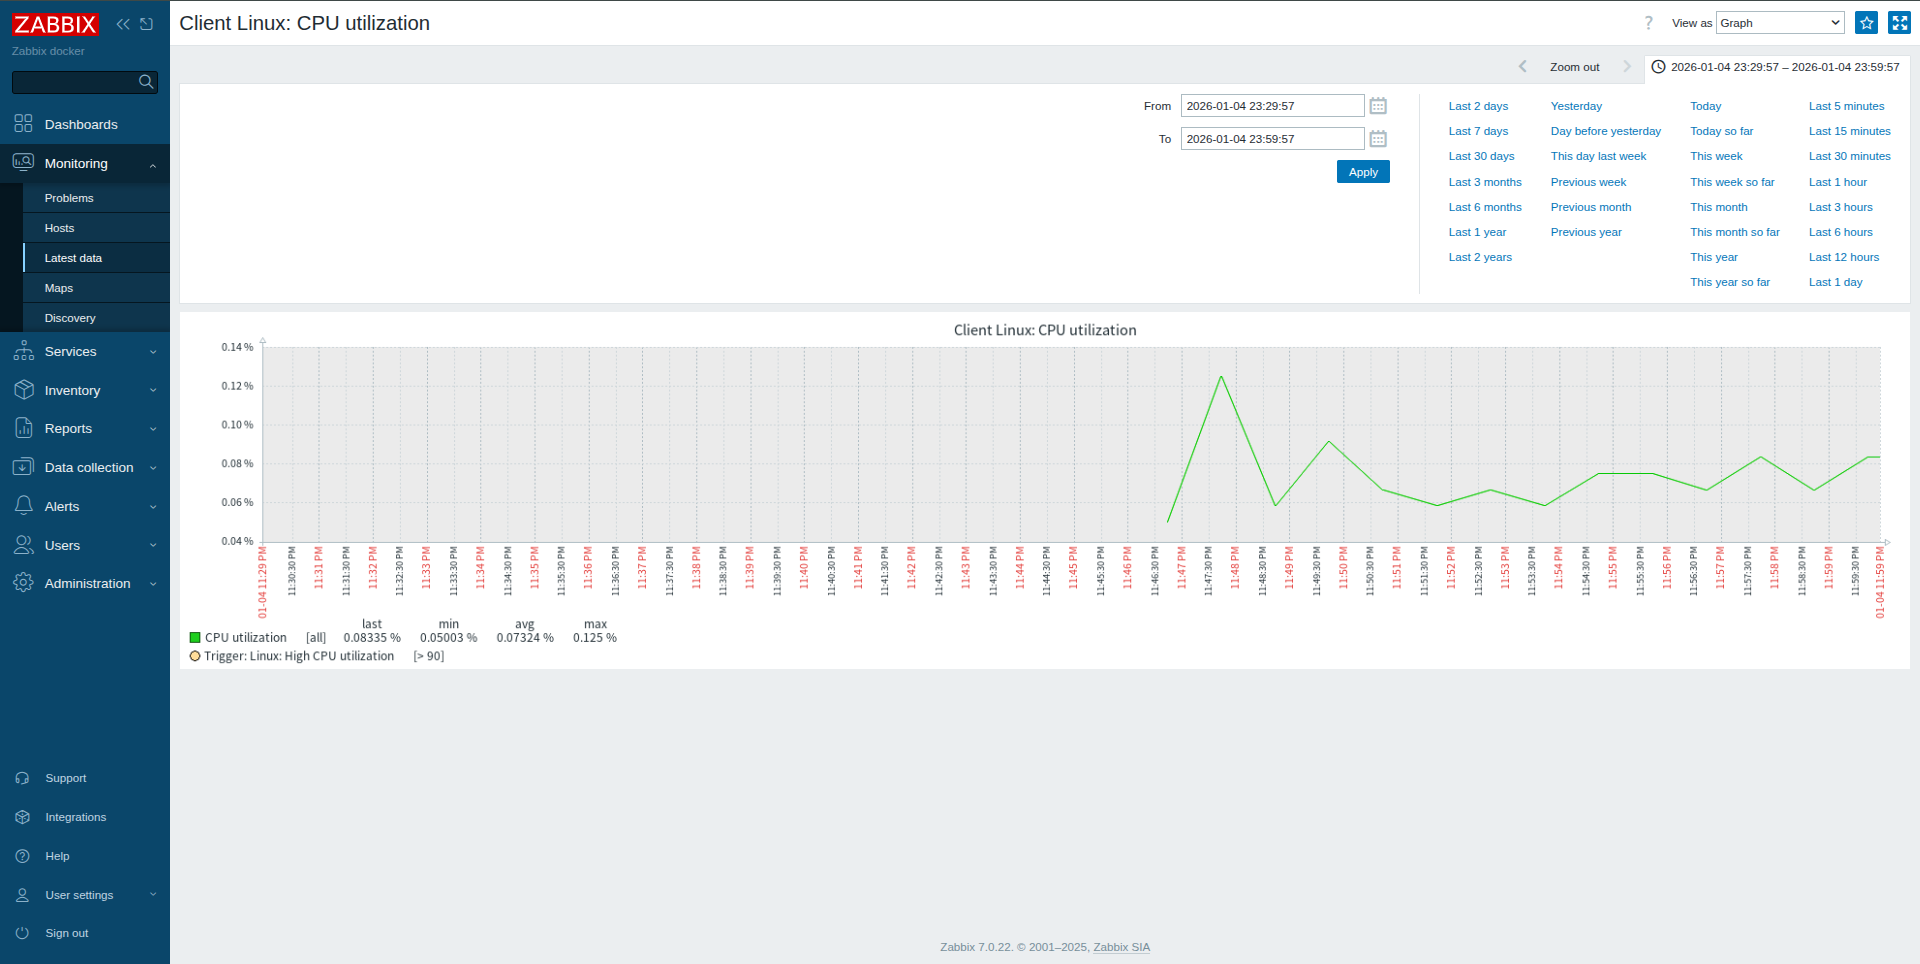
\includegraphics[width=0.95\textwidth]{images/26-zabbix-monitoring-dashboard.png}
\caption{Dashboard de monitoring Zabbix}
\label{fig:monitoring-dashboard}
\end{figure}

\section{Métriques Collectées}

\subsection{Métriques Système Linux}

Le template "Linux by Zabbix agent" collecte automatiquement :

\begin{table}[H]
\centering
\caption{Métriques Linux collectées}
\label{tab:linux-metrics}
\begin{tabular}{|l|p{8cm}|}
\hline
\textbf{Catégorie} & \textbf{Métriques} \\
\hline
CPU & Utilisation, load average, temps utilisateur/système \\
\hline
Mémoire & RAM utilisée/libre, swap, cache \\
\hline
Disque & Espace utilisé, I/O, inodes \\
\hline
Réseau & Trafic entrant/sortant, erreurs, paquets \\
\hline
Processus & Nombre de processus, zombies \\
\hline
Système & Uptime, hostname, version OS \\
\hline
\end{tabular}
\end{table}

\subsection{Métriques Système Windows}

Le template "Windows by Zabbix agent" collecte :

\begin{table}[H]
\centering
\caption{Métriques Windows collectées}
\label{tab:windows-metrics}
\begin{tabular}{|l|p{8cm}|}
\hline
\textbf{Catégorie} & \textbf{Métriques} \\
\hline
CPU & Utilisation par cœur, temps processeur \\
\hline
Mémoire & Mémoire physique, mémoire virtuelle, page file \\
\hline
Disque & Espace disque, temps de lecture/écriture \\
\hline
Réseau & Bande passante, erreurs d'interface \\
\hline
Services & État des services Windows \\
\hline
Événements & Logs Windows (Système, Application) \\
\hline
\end{tabular}
\end{table}

\section{Test de Charge (Stress Test)}

\subsection{Objectif}

Pour démontrer la capacité de Zabbix à détecter les anomalies, nous effectuons un test de charge CPU sur le client Linux.

\subsection{Exécution du Test}

\begin{lstlisting}[language=bash, caption=Installation et exécution de stress]
# Installation de l'outil stress
sudo apt install -y stress

# Lancement du stress test CPU (4 coeurs pendant 60s)
stress --cpu 4 --timeout 60s
\end{lstlisting}

\begin{figure}[H]
\centering
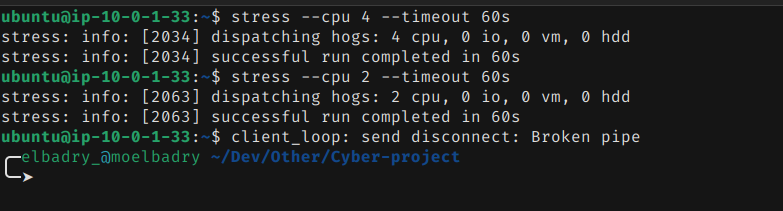
\includegraphics[width=0.95\textwidth]{images/27-stress-test-command.png}
\caption{Exécution de la commande stress}
\label{fig:stress-command}
\end{figure}

\subsection{Observation dans Zabbix}

Le pic de CPU est immédiatement visible dans les graphiques Zabbix :

\begin{figure}[H]
\centering
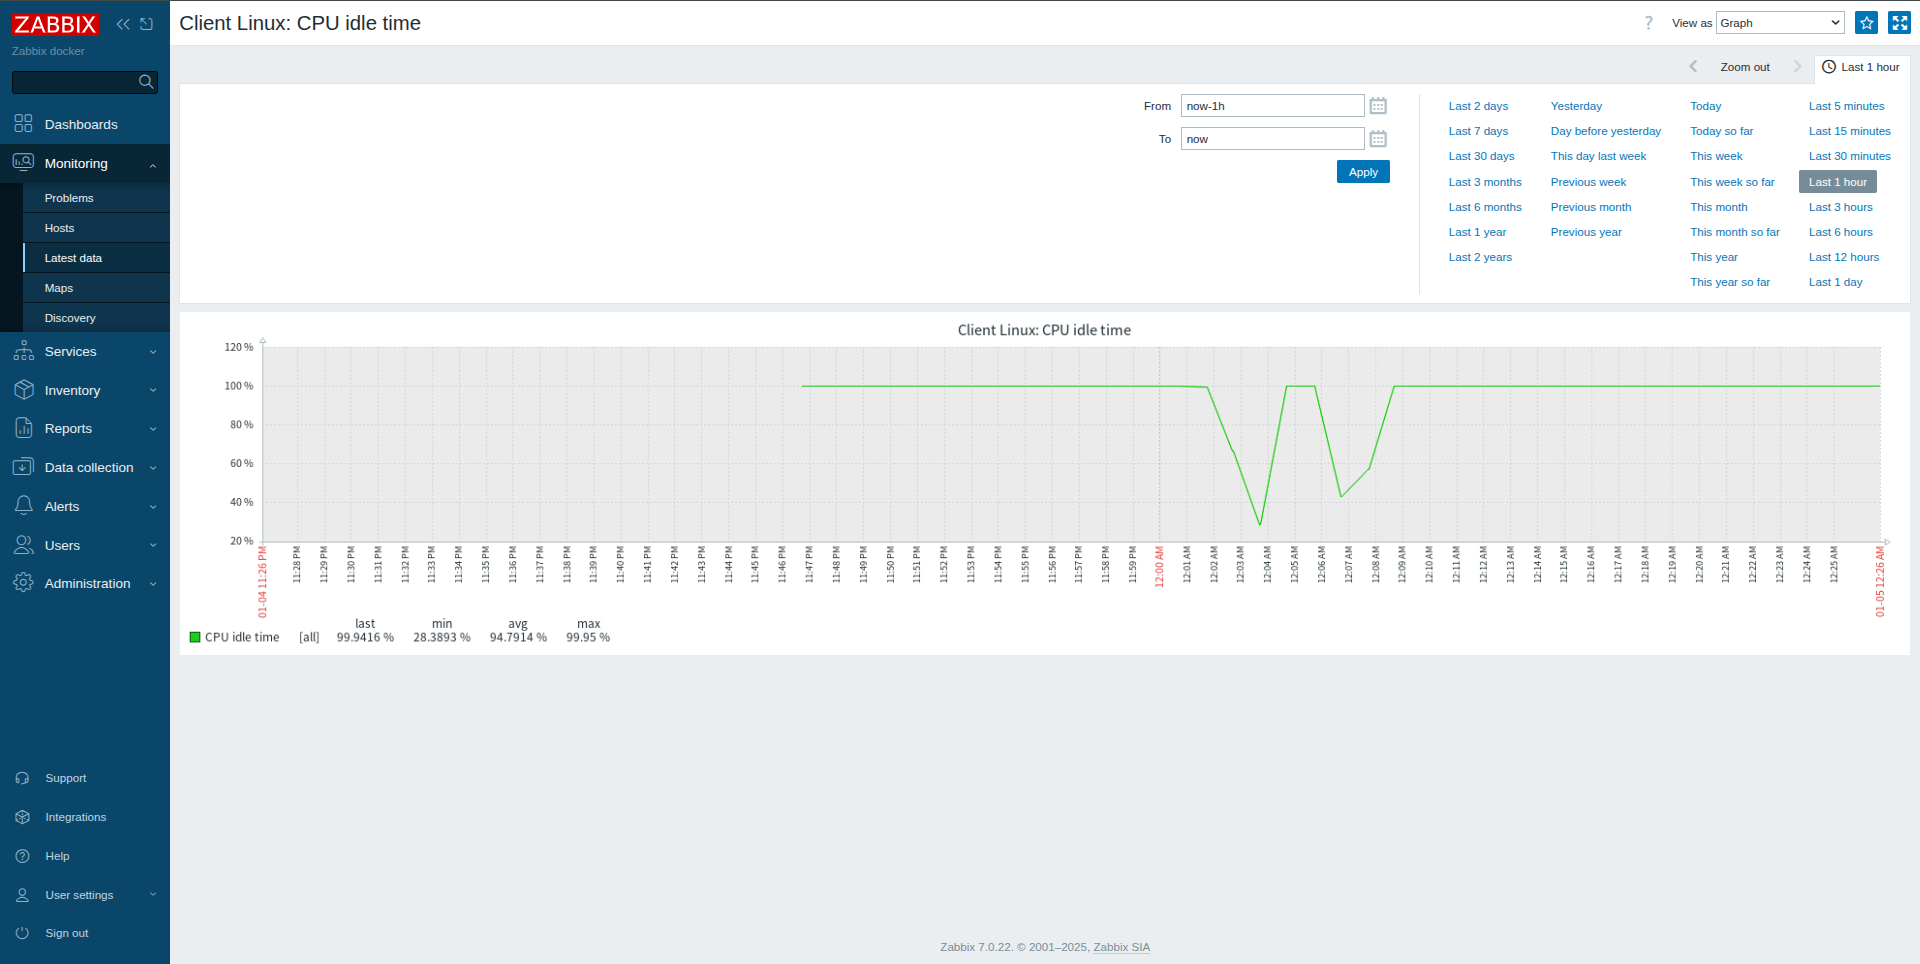
\includegraphics[width=0.95\textwidth]{images/28-stress-test-cpu-spike.png}
\caption{Pic de CPU détecté suite au stress test}
\label{fig:cpu-spike}
\end{figure}

\section{Gestion des Alertes}

\subsection{Problèmes Détectés}

Zabbix déclenche automatiquement des alertes basées sur les triggers prédéfinis :

\begin{figure}[H]
\centering
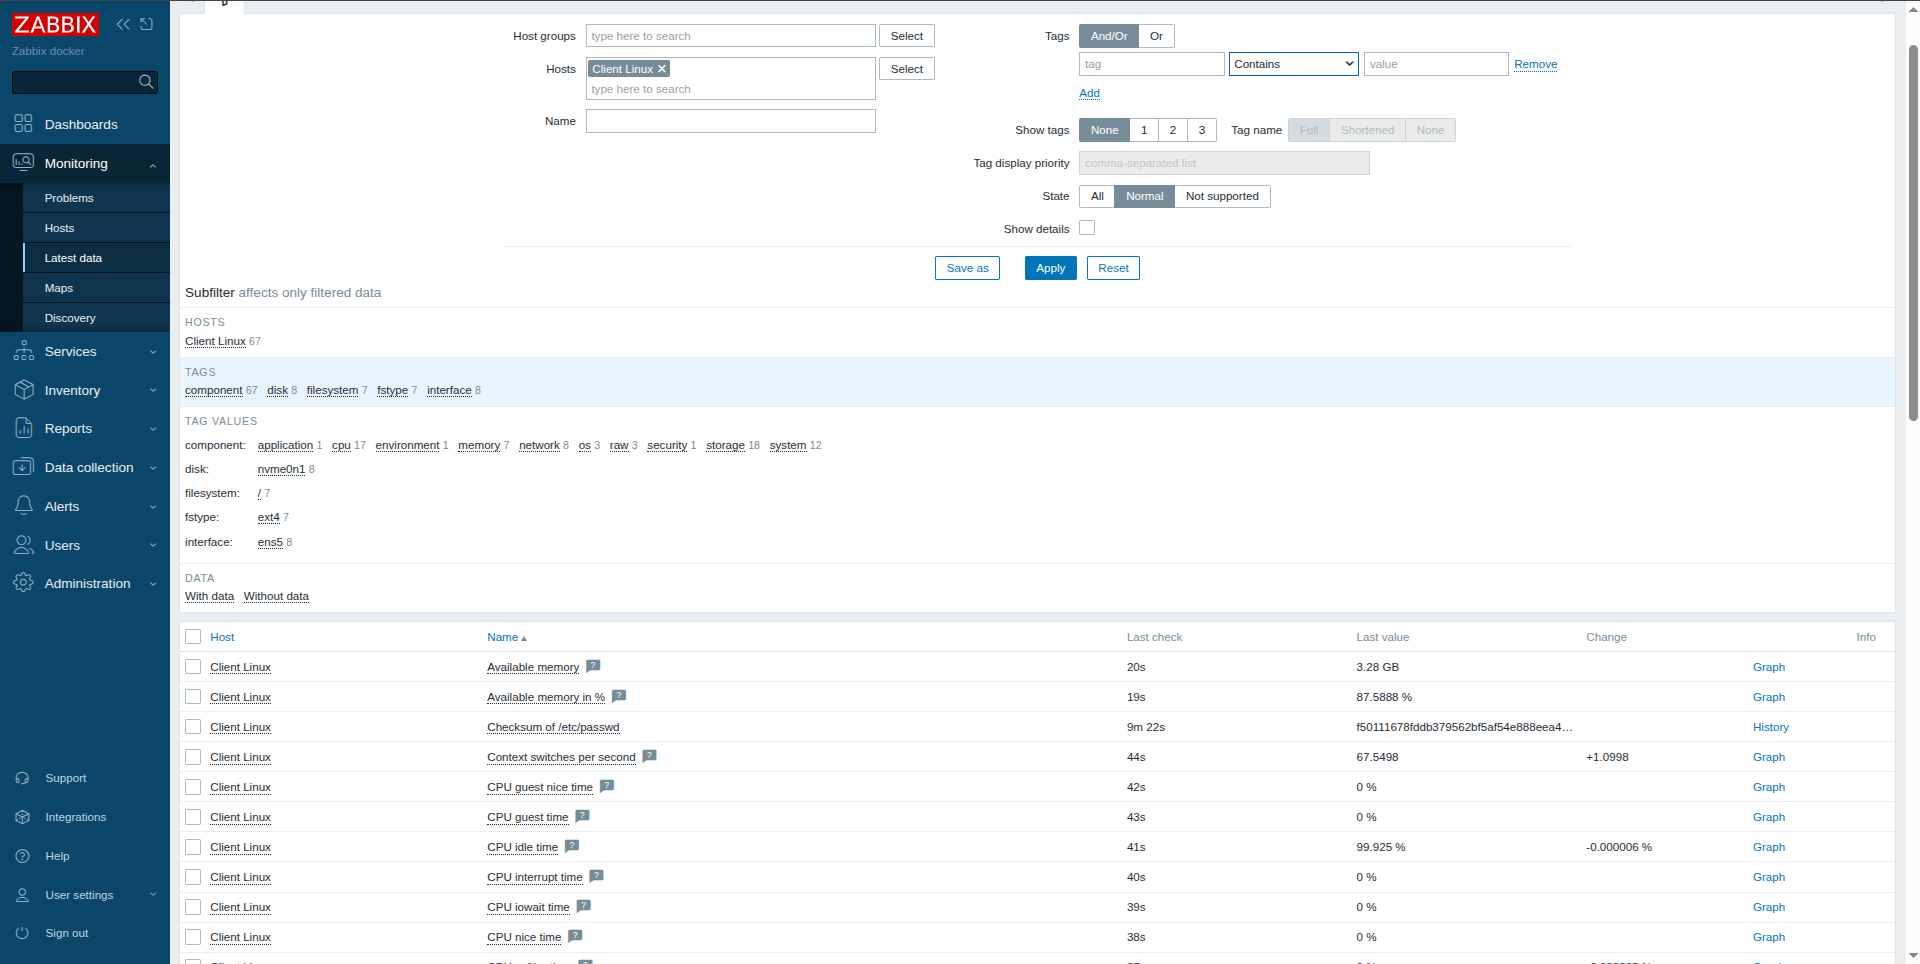
\includegraphics[width=0.95\textwidth]{images/29-zabbix-monitoring-problems.png}
\caption{Vue des problèmes actifs dans Zabbix}
\label{fig:monitoring-problems}
\end{figure}

\subsection{Liste des Problèmes}

\begin{figure}[H]
\centering
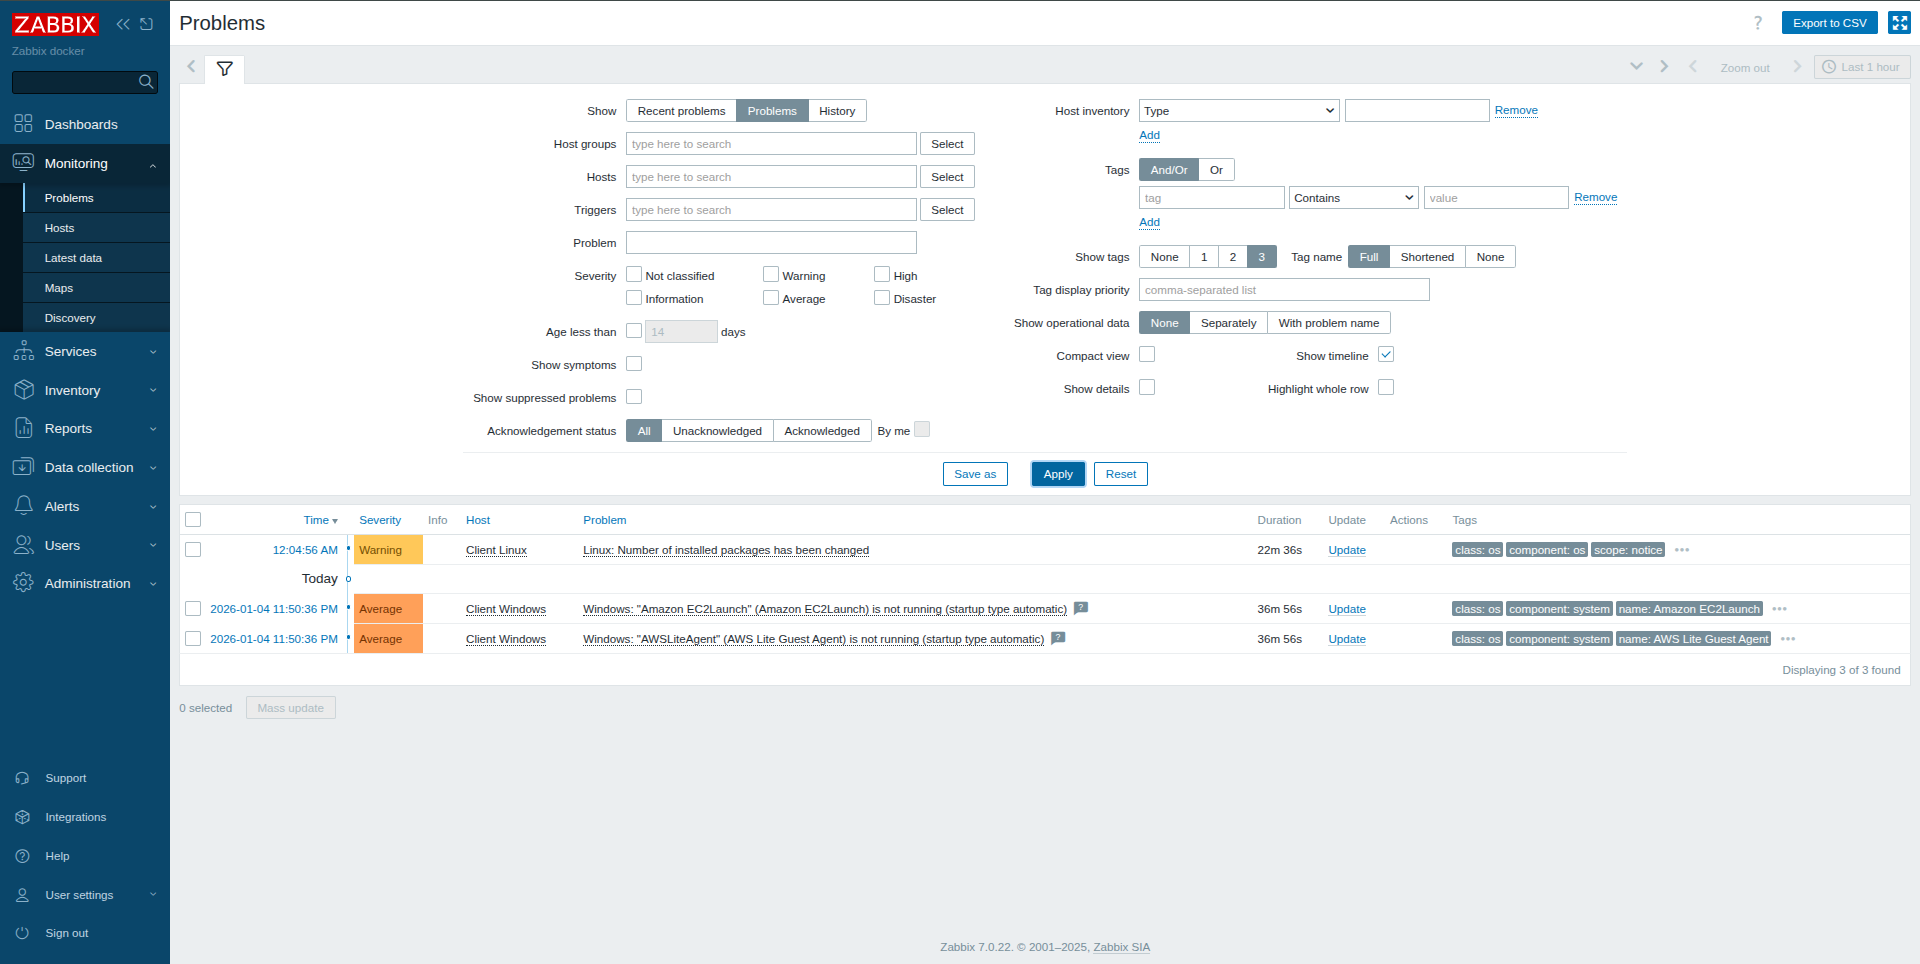
\includegraphics[width=0.95\textwidth]{images/30-zabbix-problems-list.png}
\caption{Liste détaillée des problèmes}
\label{fig:problems-list}
\end{figure}

\subsection{Historique des Événements}

L'historique complet des événements est disponible :

\begin{figure}[H]
\centering
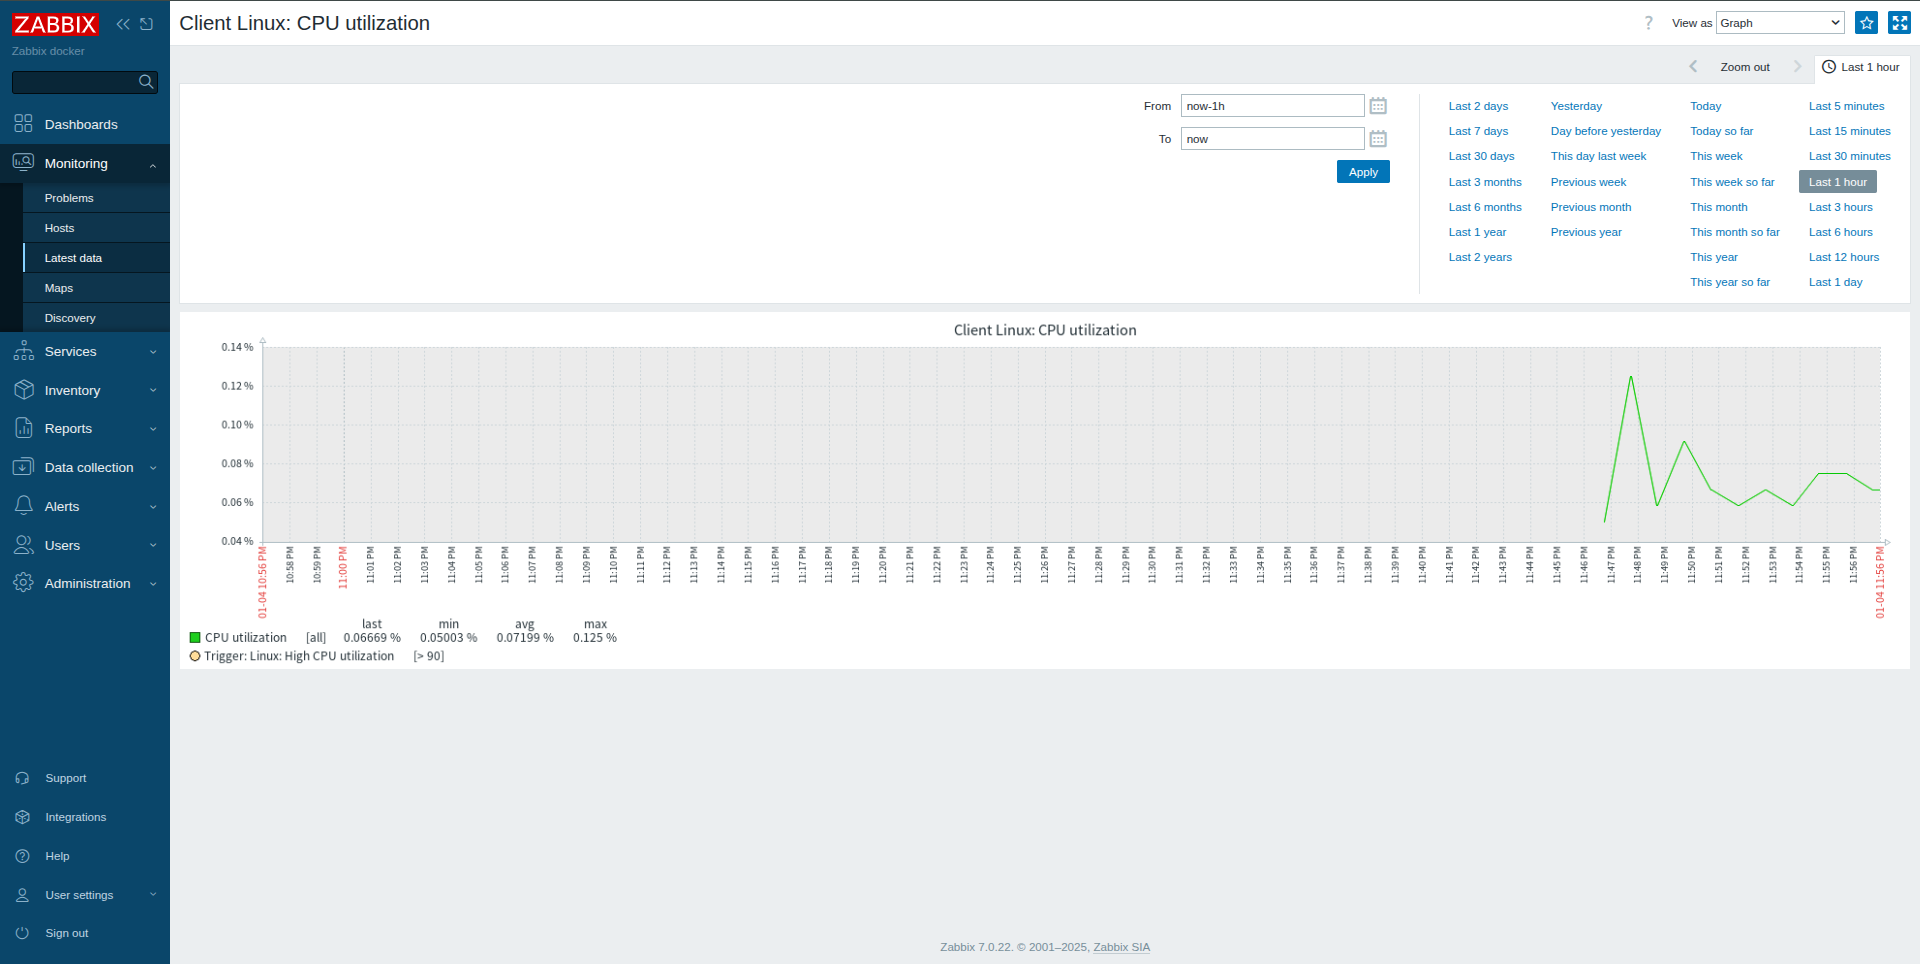
\includegraphics[width=0.95\textwidth]{images/31-zabbix-events-history.png}
\caption{Historique des événements Zabbix}
\label{fig:events-history}
\end{figure}

\section{Configuration des Triggers}

\subsection{Liste des Triggers}

Les triggers définissent les conditions de déclenchement des alertes :

\begin{figure}[H]
\centering
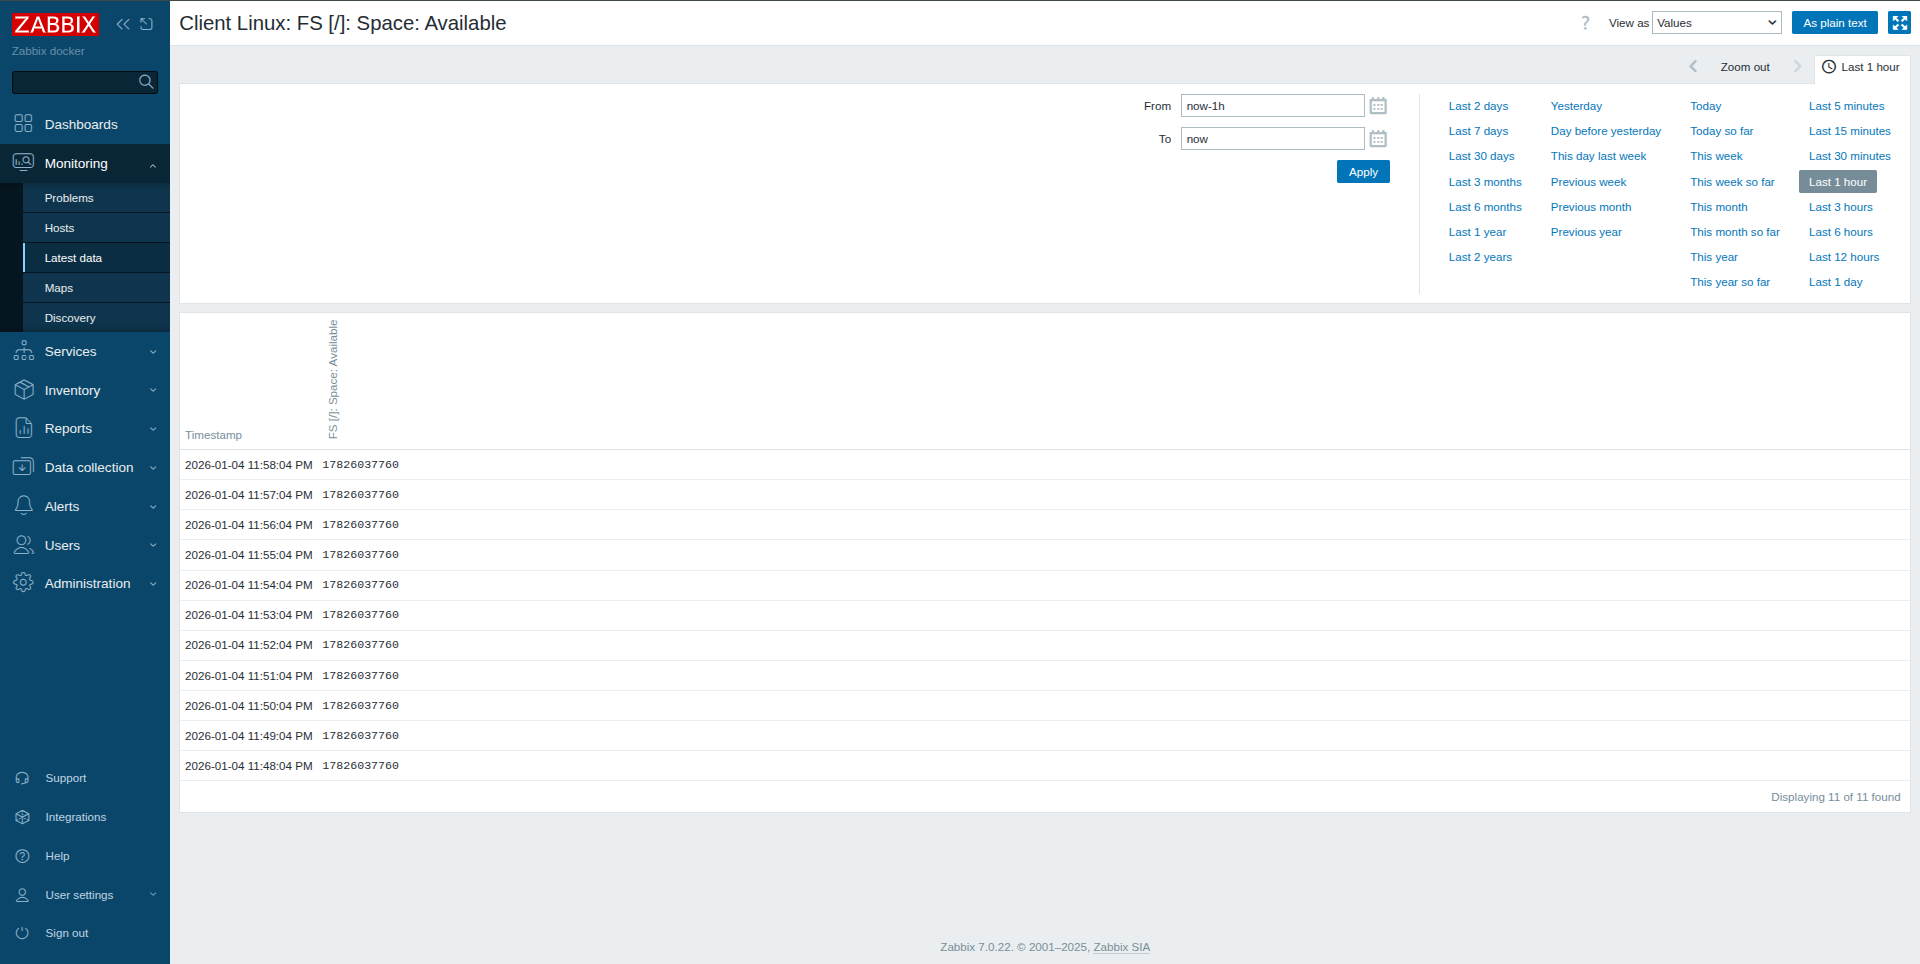
\includegraphics[width=0.95\textwidth]{images/32-zabbix-triggers-list.png}
\caption{Liste des triggers configurés}
\label{fig:triggers-list}
\end{figure}

\subsection{Exemples de Triggers}

\begin{table}[H]
\centering
\caption{Exemples de triggers Zabbix}
\label{tab:triggers-examples}
\begin{tabular}{|l|l|l|}
\hline
\textbf{Trigger} & \textbf{Sévérité} & \textbf{Condition} \\
\hline
High CPU utilization & Warning & CPU > 80\% pendant 5 min \\
\hline
High memory utilization & Warning & RAM > 90\% \\
\hline
Disk space critical & High & Espace disque < 10\% \\
\hline
Agent unreachable & Disaster & Pas de réponse pendant 3 min \\
\hline
\end{tabular}
\end{table}

\begin{figure}[H]
\centering
\includegraphics[width=0.95\textwidth]{images/33-zabbix-triggers-config.png}
\caption{Configuration d'un trigger}
\label{fig:triggers-config}
\end{figure}

\section{Visualisation des Données}

\subsection{Latest Data}

La section "Latest data" affiche les dernières valeurs collectées pour chaque métrique :

\begin{itemize}
    \item \textbf{Monitoring → Latest data}
    \item Filtrer par hôte ou groupe
    \item Voir les valeurs en temps réel
    \item Accéder aux graphiques historiques
\end{itemize}

\subsection{Graphiques}

Zabbix génère automatiquement des graphiques pour visualiser l'évolution des métriques dans le temps :

\begin{itemize}
    \item Graphiques CPU (utilisation, load)
    \item Graphiques mémoire (utilisée, libre)
    \item Graphiques réseau (trafic in/out)
    \item Graphiques disque (espace, I/O)
\end{itemize}

\section{Récapitulatif du Monitoring}

\begin{table}[H]
\centering
\caption{État final du monitoring}
\label{tab:monitoring-summary}
\begin{tabular}{|l|c|c|c|}
\hline
\textbf{Hôte} & \textbf{Statut} & \textbf{Template} & \textbf{Items} \\
\hline
Zabbix-Server & \textcolor{green}{ZBX} & Linux by Zabbix agent & ~150 \\
\hline
ELBadry-Client-Linux & \textcolor{green}{ZBX} & Linux by Zabbix agent & ~150 \\
\hline
ELBadry-Client-Windows & \textcolor{green}{ZBX} & Windows by Zabbix agent & ~200 \\
\hline
\end{tabular}
\end{table}

\section{Points Clés}

\begin{itemize}
    \item[$\checkmark$] Les 3 hôtes sont supervisés avec succès (ZBX vert)
    \item[$\checkmark$] Les métriques sont collectées en temps réel
    \item[$\checkmark$] Le stress test a déclenché les alertes appropriées
    \item[$\checkmark$] Les graphiques affichent l'historique des performances
    \item[$\checkmark$] Les triggers fonctionnent correctement
\end{itemize}
